\documentclass[11pt]{article}

% LiveShark — minimal "premium product" style (printable, sober)

\usepackage[a4paper,margin=2.3cm]{geometry}

% Fonts: modern, readable, widely available in TeX Live
\usepackage{fontspec}
\setmainfont{DejaVu Serif}
\setsansfont{DejaVu Sans}

\usepackage{microtype}

% Color palette (subtle)
\usepackage{xcolor}
\definecolor{LSBlue}{HTML}{1A355E}
\definecolor{LSGray}{HTML}{F4F6F8}
\definecolor{LSMid}{HTML}{5B6675}

% Headings
\usepackage{titlesec}
\titleformat{\section}{\sffamily\bfseries\Large\color{LSBlue}}{\thesection}{0.8em}{}
\titleformat{\subsection}{\sffamily\bfseries\large\color{LSBlue}}{\thesubsection}{0.8em}{}
\titleformat{\subsubsection}{\sffamily\bfseries\normalsize\color{LSBlue}}{\thesubsubsection}{0.8em}{}
\titlespacing*{\section}{0pt}{2.0ex}{1.1ex}
\titlespacing*{\subsection}{0pt}{1.6ex}{0.9ex}

% Lists
\usepackage{enumitem}
\setlist[itemize]{leftmargin=*,topsep=0.4em,itemsep=0.25em}
\setlist[enumerate]{leftmargin=*,topsep=0.4em,itemsep=0.25em}

% Tables
\usepackage{booktabs}
\usepackage{tabularx}
\renewcommand{\arraystretch}{1.15}

% Links: NO red boxes
\usepackage[hidelinks]{hyperref}
\hypersetup{
  colorlinks=true,
  linkcolor=LSBlue,
  urlcolor=LSBlue,
  citecolor=LSBlue,
  pdfborder={0 0 0}
}

% Header/footer
\usepackage{fancyhdr}
\pagestyle{fancy}
\fancyhf{}
\renewcommand{\headrulewidth}{0.2pt}
\renewcommand{\footrulewidth}{0pt}
\fancyhead[L]{\sffamily\small\color{LSMid}\lsProjectTitle}
\fancyhead[R]{\sffamily\small\color{LSMid}\lsSpecStatus}
\fancyfoot[C]{\sffamily\small\color{LSMid}\thepage}

% Figures
\usepackage{graphicx}
\usepackage{caption}
\captionsetup{labelfont={sf,bf},textfont=sf,font=small}

% TikZ (for clean diagrams) — kept simple
\usepackage{tikz}
\usetikzlibrary{arrows.meta,positioning,shapes,fit}
\usepackage{adjustbox}

% Framed boxes for requirements/notes (subtle)
\usepackage[most]{tcolorbox}
\tcbset{
  colback=LSGray,
  colframe=LSBlue!35,
  arc=2mm,
  boxrule=0.4pt,
  left=1.4mm,right=1.4mm,top=1.0mm,bottom=1.0mm
}

% Project variables
\newcommand{\lsProjectTitle}{LiveShark — Specification}
\newcommand{\lsSpecStatus}{DRAFT}

% RFC 2119 keywords helpers (visual emphasis, not noisy)
\newcommand{\MUST}{\textbf{MUST}}
\newcommand{\MUSTNOT}{\textbf{MUST NOT}}
\newcommand{\SHOULD}{\textbf{SHOULD}}
\newcommand{\SHOULDNOT}{\textbf{SHOULD NOT}}
\newcommand{\MAY}{\textbf{MAY}}

% Requirement box (ID + priority)
\newtcolorbox{reqbox}[3]{title=\sffamily\bfseries #1 \hfill \sffamily #2, colback=LSGray, colframe=LSBlue!45}
% #1 = ID, #2 = Priority, #3 = (unused placeholder to allow future extensions)


\usepackage{csquotes}
\usepackage{biblatex}
\addbibresource{../common/references.bib}

\title{\sffamily\bfseries\color{LSBlue}LiveShark\\\large Specification (Printable PDF) v0.1}
\author{\sffamily Florian Keller}
\date{\sffamily Draft - \today\\\small\textsf{Authoritative language: EN}}

\begin{document}
\maketitle
\vspace{0.6em}

\begin{tcolorbox}
\textbf{Scope.} LiveShark is a \textbf{passive} analyzer for show-control networking (Art-Net, sACN). It focuses on
\textbf{offline PCAP analysis} with \textbf{DMX frame reconstruction}, \textbf{automatic conflict detection},
and \textbf{reproducible reports}.\\
\textbf{Audience.} Designed to be readable by \textbf{non-software specialists} (lighting technicians, integrators, QA).
Planned \textbf{follow mode} enables near-real-time analysis of a capture file that is still being written by an external tool.\\
The ideal user interface is a well-designed \textbf{GUI}; the \textbf{CLI} remains scriptable and produces the same report data.
\end{tcolorbox}

\newpage
\tableofcontents
\newpage

\section{Terminology and conventions}

\subsection{Authoritative version and translation policy}
\textbf{Authoritative version (prevails).} The English specification in \texttt{spec/en} is the \emph{authoritative}
version: in case of discrepancy or incomplete translation, \textbf{the English version prevails}.\\
\textbf{French translation (informational).} A French translation may exist in \texttt{spec/fr}. It is provided as a convenience and
\textbf{may lag behind}. When differences exist, the authoritative version prevails.

\subsection{Normative keywords}
The key words \MUST, \MUSTNOT, \SHOULD, \SHOULDNOT, and \MAY{} are to be interpreted as described in BCP 14
(RFC 2119 and RFC 8174). Only \textbf{UPPERCASE} usage is normative.

\subsection{Implementation language note}
LiveShark is implemented in \textbf{Rust} to balance \textbf{memory safety}, \textbf{performance}, and \textbf{cross-platform}
delivery (Windows, macOS, Linux) with a modern toolchain. This is an engineering choice for v0.1 and does not preclude
future components from using other languages where justified.
Rust code SHOULD follow the standard Rust style guide: \texttt{https://doc.rust-lang.org/style-guide/}.


\subsection{Term note: \enquote{Live}}
In the project name, \enquote{Live} refers to \textbf{live entertainment / show control} (lighting networks), not to a guarantee
of real-time capture capability. Real-time capture is optional and may be introduced in later releases.
Near-real-time diagnostic can be achieved via follow mode without requiring native live capture.

\subsection{Core terms}
\begin{adjustbox}{max width=\linewidth}
\begin{tabularx}{\linewidth}{@{}l >{\raggedright\arraybackslash}X@{}}
\toprule
\textbf{Term} & \textbf{Meaning} \\
\midrule
Packet & Network packet as captured in PCAP/PCAPNG. \\
Protocol message & Decoded application-layer unit (e.g., ArtDMX,\\ sACN Data Packet). \\
DMX frame & Reconstructed DMX512 state (512 slots) for a universe at a given time. \\
Universe & Logical group of up to 512 DMX slots. \\
Source & Emitter identified by IP and, if applicable, protocol identity (e.g., sACN CID). \\
Flow & Unidirectional tuple (proto, src ip:port, dst ip:port). \\
\bottomrule
\end{tabularx}
\end{adjustbox}

\subsection{Acronyms}
\begin{adjustbox}{max width=\linewidth}
\begin{tabularx}{\linewidth}{@{}l >{\raggedright\arraybackslash}X@{}}
\toprule
\textbf{Acronym} & \textbf{Expanded form} \\
\midrule
ArtDMX & Art-Net DMX data packet \\
Art-Net & Art-Net lighting control protocol \\
BCP & Best Current Practice \\
CC-BY-4.0 & Creative Commons Attribution 4.0 International \\
CID & Component Identifier (sACN source identifier) \\
CI & Continuous integration \\
CLI & Command-line interface \\
DMX & Digital Multiplex (DMX512 / DMX512-A) \\
DMX512 & Digital Multiplex 512 \\
DoD & Definition of Done \\
FPS / PPS / BPS & Frames / Packets / Bytes per second \\
GUI & Graphical user interface \\
IP & Internet Protocol \\
JSON & JavaScript Object Notation \\
MIT & Massachusetts Institute of Technology (license) \\
MVP & Minimum Viable Product \\
PCAP & Packet Capture file format \\
PCAPNG & PCAP Next Generation file format \\
QA & Quality assurance \\
RFC & Request for Comments \\
sACN & Streaming ACN (ANSI E1.31) \\
UDP & User Datagram Protocol \\
\bottomrule
\end{tabularx}
\end{adjustbox}

\section{What LiveShark is (and is not)}

\subsection{Goals}
\begin{itemize}
  \item Offline analysis of PCAP/PCAPNG for Art-Net and sACN.
  \item DMX frame reconstruction (512 slots) and metrics (fps, pps/bps, jitter, loss, bursts).
  \item Automatic detection of \textbf{conflicts} (multiple sources on same universe with overlap).
  \item Versioned, reproducible JSON reports for tickets, post-mortem, QA and CI.
\end{itemize}
See Appendices A--D for the normative contracts (report, frames, conflicts, metrics).

\paragraph{Capture input (no Wireshark required).}
LiveShark \MUSTNOT{} require the Wireshark GUI\\ application to operate.
For v0.1, captures are provided as PCAP/PCAPNG files produced by standard tools (e.g., \texttt{tcpdump} on Linux,\\
\texttt{pktmon} on Windows, or any capture tool that exports PCAP/PCAPNG).
Live capture is a future objective and \MAY{} be added later via libpcap/Npcap (without changing the report schema).



\subsection{Offline-first strategy (product intent)}
LiveShark is designed as an \emph{offline-first} analyzer:\\
early releases focus on post-mortem analysis of PCAP/PCAPNG captures
to maximize robustness, reproducibility, and ease of support. This is a deliberate engineering strategy, not a product limitation.
Live capture / online analysis is an explicit future objective and \MAY{} be implemented once the offline core is validated.

\textbf{Forward compatibility.} The core analysis pipeline \MUST{} be architected so that packet input can come from either:
(a) a file reader (PCAP/PCAPNG), or (b) a live capture source (future). No offline-only assumption \MUST{} be embedded in the
domain model (frames, conflicts, reports).

Follow mode is the pragmatic path for reliable diagnostics during show preparation and during the show: it analyzes a capture
file as it grows, without requiring native capture on day one.

LiveShark may emit \emph{probable-cause hints} only as heuristics and separate from measured metrics. Any hint \MUST{} be
justified by observable indicators (loss patterns, jitter, bursts, timing asymmetries) and \MUSTNOT{} be presented as a certain
cause. Robust loss localization may require multiple capture points (for example, before and after a wireless segment) and is
reported only when feasible based on the available evidence.



\subsection{Non-goals}
\begin{itemize}
  \item LiveShark is \textbf{not} a general-purpose packet analyzer (it does not replace Wireshark).
  \item LiveShark is \textbf{passive} by design: it does not transmit or inject traffic.
  \item ``Laser over IP'' starts as \textbf{generic UDP flow metrics only}; laser frame reconstruction is out of scope for v0.1.
\end{itemize}

\subsection{Optional extensions (non-normative register)}
LiveShark is designed for diagnostics. Extensions must improve actionable diagnosis (loss, jitter, bursts, conflicts, multi-source) and must remain reproducible (same input $\rightarrow$ same output).
These candidates are non-normative and not part of the v0.1 scope.

Each extension declares its support level:
\begin{itemize}
  \item \textbf{Flow level:} network-level metrics without payload semantics.
  \item \textbf{Message/Frame level:} structured decoding with a stable domain model.
\end{itemize}

LiveShark may emit \emph{probable-cause hints} only as heuristics. Such hints must be justified by observable patterns and must never be presented as certain causes.

  \begin{itemize}
    \item \textbf{OSC (Message):} control-message timeline; correlation with DMX/network anomalies.
    \item \textbf{RTP-based protocols (Message):} sequence gaps, jitter, reordering; basis for health checks (e.g., AES67).
    \item \textbf{Network infrastructure (Flow):} IGMP/mDNS/DHCP/ARP/DNS patterns; multicast/discovery/addressing issues.
  \end{itemize}

\section{Architecture (conceptual)}
\begin{figure}[H]
\centering
\begin{adjustbox}{max width=\linewidth}
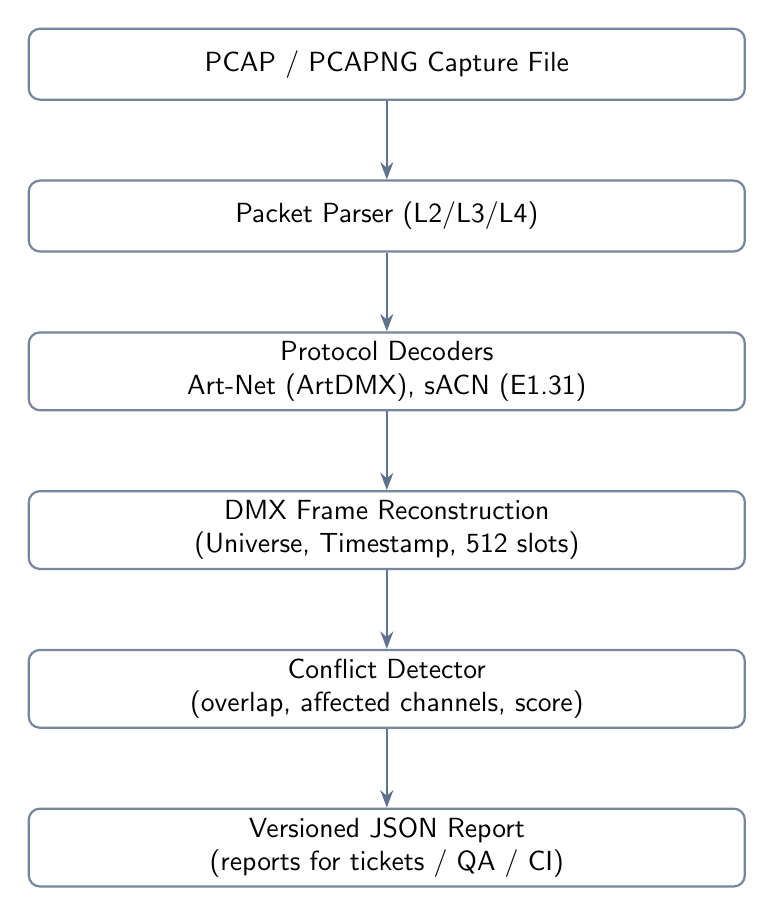
\begin{tikzpicture}[
  node distance=10mm,
  box/.style={rounded corners, draw=LSBlue!60, fill=white, thick, minimum width=0.75\linewidth, minimum height=9mm, align=center, font=\sffamily},
  arrow/.style={-{Stealth[length=2.2mm]}, thick, draw=LSBlue!70},
]
\node[box] (pcap) {PCAP / PCAPNG Capture File};
\node[box, below=of pcap] (parse) {Packet Parser (L2/L3/L4)};
\node[box, below=of parse] (decode) {Protocol Decoders \\ Art-Net (ArtDMX), sACN (E1.31)};
\node[box, below=of decode] (frame) {DMX Frame Reconstruction \\ (Universe, Timestamp, 512 slots)};
\node[box, below=of frame] (conf) {Conflict Detector \\ (overlap, affected channels, score)};
\node[box, below=of conf] (report) {Versioned JSON Report \\ (reports for tickets / QA / CI)};
\draw[arrow] (pcap) -- (parse);
\draw[arrow] (parse) -- (decode);
\draw[arrow] (decode) -- (frame);
\draw[arrow] (frame) -- (conf);
\draw[arrow] (conf) -- (report);
\end{tikzpicture}

\end{adjustbox}
\caption{Conceptual offline analysis pipeline (high level).}
\textit{Note:} The pipeline currently accepts (v0.1) only PCAP/PCAPNG files. Live capture input is a future objective (v0.3+),
aligned with the input abstraction requirement in P0.
\end{figure}

\section{Metrics (defaults)}
Unless otherwise stated:
\begin{itemize}
  \item \textbf{pps/bps window:} 1.0 s sliding window
  \item \textbf{fps window:} 5.0 s sliding window
  \item \textbf{jitter window:} 10.0 s sliding window (see metrics definition; concept reference: RFC 3550)
\end{itemize}

\subsection{Metrics definitions (minimal)}
\begin{itemize}
  \item \textbf{pps/bps:} packets/bytes per second over a 1.0 s sliding window.
  \item \textbf{fps (universe):} reconstructed DMX frames per second over a 5.0 s sliding window.
  \item \textbf{jitter (IAT):} population standard deviation of inter-arrival time deltas over a 10.0 s sliding window (RFC 3550 \S6.4.1). Formula: $\sigma = \sqrt{\frac{1}{n}\sum(\Delta_i - \mu)^2}$ with $\Delta_i = t_i - t_{i-1}$.
  \item \textbf{loss (observed):} when protocol sequence numbers exist (e.g., sACN), loss is reported as observed sequence gaps at the capture point. In v0.1, loss \MUST{} be reported only when sequence numbers exist; otherwise loss fields are omitted. This does not guarantee loss at the receiver.
\end{itemize}
See Appendix D for operational definitions and units.

\section{Contractual requirements (extract)}
This document is a bootstrap spec: requirements are intentionally minimal at project start.

\subsection{Priority P0 (MVP foundations)}
\begin{reqbox}{LS-ARCH-001}{P0}{}
The core \MUST{} expose a packet/event input abstraction so that analysis can be driven by:
(a) a PCAP/PCAPNG file reader (v0.1), and (b) a live capture source (future), without changing the domain model or report schema.
\end{reqbox}

\begin{reqbox}{LS-PROD-001}{P0}{}
LiveShark \MUSTNOT{} require the Wireshark GUI application. It \MUST{} accept PCAP/PCAPNG files produced by standard capture tools.
\end{reqbox}

\begin{reqbox}{LS-FR-001}{P0}{}
LiveShark \MUST{} ingest PCAP/PCAPNG files and enumerate UDP flows.
\end{reqbox}

\begin{reqbox}{LS-FR-010}{P0}{}
LiveShark \MUST{} decode Art-Net ArtDMX and reconstruct DMX frames (512 slots) per universe.
\end{reqbox}

\begin{reqbox}{LS-FR-011}{P0}{}
LiveShark \MUST{} decode sACN (E1.31) DMX data packets and reconstruct DMX frames per universe.
\end{reqbox}

\subsection{Priority P1 (critical differentiators)}
\begin{reqbox}{LS-CONF-001}{P1}{}
LiveShark \MUST{} detect concurrent sources: two or more sources emitting on the same universe with overlap $> 1.0$ s.
\end{reqbox}

\begin{reqbox}{LS-REP-001}{P1}{}
LiveShark \MUST{} generate a versioned JSON report containing at least: capture summary, universes (with per-universe sources),
flows, and conflicts.
\end{reqbox}

\begin{reqbox}{LS-REP-002}{P1}{}
The JSON report \MUST{} be deterministic: list ordering is stable and all volatile fields are explicitly defined.
\end{reqbox}

\begin{reqbox}{LS-REP-003}{P1}{}
The JSON report \MUST{} include the minimal schema fields and types defined in Appendix A (v0.1).
\end{reqbox}

\begin{reqbox}{LS-REP-004}{P1}{}
Conflict records in the JSON report \MUST{} follow the structure defined in Appendix C.
\end{reqbox}

\begin{reqbox}{LS-FR-012}{P0}{}
LiveShark \MUST{} use a canonical reconstructed DMX frame definition (fields + 512 slots) as defined in Appendix B.
\end{reqbox}

\begin{reqbox}{LS-FR-013}{P1}{}
LiveShark \MUST{} follow the frame reconstruction rules and fps counting rules defined in Appendix B.
\end{reqbox}

\begin{reqbox}{LS-CONF-002}{P1}{}
LiveShark \MUST{} use the source identity definition for conflicts defined in Appendix C.
\end{reqbox}

\begin{reqbox}{LS-CONF-003}{P1}{}
LiveShark \MUST{} compute overlap for conflicts using the definition in Appendix C.
\end{reqbox}

\begin{reqbox}{LS-CONF-010}{P1}{}
LiveShark \MUST{} use the source identity definition for conflict detection defined in Appendix C (CID + fallback).
\end{reqbox}

\begin{reqbox}{LS-CONF-011}{P1}{}
LiveShark \MUST{} compute conflict overlap using capture timestamps and the threshold defined in Appendix C (v0.1).
\end{reqbox}

\begin{reqbox}{LS-CONF-012}{P1}{}
Conflict records \MUST{} include the required fields defined in Appendix C (v0.1).
\end{reqbox}

\begin{reqbox}{LS-MET-001}{P1}{}
LiveShark \MUST{} compute and report pps/bps/fps/jitter as defined in Appendix D (v0.1).
\end{reqbox}
\section{Known limitations (v0.1)}
\begin{itemize}
  \item \textbf{Compliance percentage} is a placeholder (reported as 100.0) until a formal denominator is defined.
  \item \textbf{Conflict detection} uses time overlap only and may produce false positives when sources are active on different channels. The false-positive rate is not quantified in v0.1; conflicts are signals to investigate.
  \item \textbf{sACN validation} drops packets with non-zero start code or invalid property value count.
\end{itemize}
\section{Validation criteria (extract)}

\subsection{Definition of Done v0.1}
The MVP is considered delivered if:
\begin{enumerate}
  \item \texttt{liveshark pcap analyse --report out/report.json file.pcapng}\\
  runs successfully on 3 captures.
  \item Art-Net and sACN are decoded (universes, sources, fps).
  \item The JSON report contains \texttt{conflicts[]} (automatic detection).
  \item No crash occurs on truncated/corrupted PCAPs.
\end{enumerate}

\subsection{Validation checklist (report contract)}
\begin{enumerate}
  \item Report includes \texttt{report\_version}, \texttt{tool}, \texttt{generated\_at}, \texttt{input}, and sections\\
  \texttt{capture\_summary}, \texttt{universes[]}, \texttt{flows[]}, \texttt{conflicts[]}, \texttt{compliance[]}.
  \item Deterministic ordering rules are applied (Appendix A).
  \item At least 4 golden tests: \texttt{artnet}, \texttt{artnet\_conflict}, \texttt{sacn}, \texttt{sacn\_conflict}.
  \item Volatile fields (\texttt{generated\_at}, and optionally \texttt{input.path}) are normalized in golden tests.
\end{enumerate}

\subsection{Golden tests}
Format: \texttt{tests/golden/<name>/\{input.pcapng, expected\_report.json,\\ metadata.toml\}}.
\texttt{metadata.toml} documents test intent, assertions (e.g., \texttt{fps\_min}, \texttt{compliance\_percentage}), and tolerance
rules. See \texttt{AGENTS.md} \S9.4 for the schema.

\appendix
\section{Appendices (Normative)}
\subsection{Appendix A --- JSON report contract (v0.1)}
\subsubsection{Minimal schema (fields and types)}
\begin{itemize}
  \item \texttt{report\_version}: integer (schema version).
  \item \texttt{tool.name} and \texttt{tool.version}: strings (tool identification).
  \item \texttt{generated\_at}: string, RFC3339 timestamp.
  \item \texttt{input.path}: string; \texttt{input.bytes}: integer.
  \item \texttt{capture\_summary}: object or null (when unavailable).
  \item \texttt{universes[]}, \texttt{flows[]}, \texttt{conflicts[]}: arrays (may be empty in v0.1).
  \item \texttt{compliance[]}: array (may be empty in v0.1).
  \item \texttt{universes[]} elements contain: \texttt{universe} (integer), \texttt{proto} (string),
  \texttt{sources[]} (array of objects with \texttt{source\_ip}, optional \texttt{cid} and \texttt{source\_name};
    \texttt{cid} is lowercase hex, 32 characters, no separators),
    \texttt{fps} (float or null), \texttt{frames\_count} (integer), and optional metric fields\\
    \texttt{loss\_packets}, \texttt{loss\_rate}, \texttt{burst\_count}, \texttt{max\_burst\_len}, \texttt{jitter\_ms}
  (omitted when unavailable).
  \item \texttt{flows[]} elements contain: \texttt{app\_proto} (string), \texttt{src} (string), \texttt{dst} (string),
  and optional \texttt{pps}, \texttt{bps}, \texttt{iat\_jitter\_ms} (omitted when unavailable).
  \item \texttt{conflicts[]} elements are defined in Appendix C.
  \item \texttt{compliance[]} elements contain: \texttt{protocol} (string), \texttt{compliance\_percentage} (float; v0.1 uses 100.0 as a placeholder),
  and \texttt{violations[]} (array of objects with: \texttt{id} (stable identifier), \texttt{severity} (string; v0.1 uses \texttt{warning} or \texttt{error}),
  \texttt{message} (human-readable explanation), \texttt{count} (integer, total number of occurrences across the capture), and optional
  \texttt{examples[]} (array of at most 3 strings, each containing concise context such as \texttt{"source IP:port @ timestamp"};\\
  payload bytes are not required).
  When present, examples \MUST{} be deduplicated, sorted stably, and limited to 3 to keep reports compact and deterministic. Examples are illustrative only and do not affect \texttt{count}.
\end{itemize}

\subsubsection{Compliance violation IDs (v0.1, non-exhaustive)}
\begin{itemize}
  \item \texttt{LS-UDP-SLICE}: UDP slice error; packet ignored.
  \item \texttt{LS-UDP-MISSING-NETWORK}: missing network layer; packet ignored.
  \item \texttt{LS-UDP-MISSING-PAYLOAD}: missing IP payload; packet ignored.
  \item \texttt{LS-UDP-TOO-SHORT}: UDP payload too short; packet ignored.
  \item \texttt{LS-ARTNET-UNIVERSE-ID}: Art-Net universe id out of range (value $> 0x7FFF$); packet ignored.
  \item \texttt{LS-ARTNET-LENGTH}: ArtDMX length invalid (0 or $> 512$); packet ignored.
  \item \texttt{LS-ARTNET-TOO-SHORT}: payload too short; packet ignored.
  \item \texttt{LS-SACN-START-CODE}: sACN start code is not 0x00; packet ignored.
  \item \texttt{LS-SACN-PROPERTY-COUNT}: sACN property value count is 0 or exceeds 512; packet ignored.
  \item \texttt{LS-SACN-DMX-LENGTH}: sACN DMX data length invalid; packet ignored.
  \item \texttt{LS-SACN-TOO-SHORT}: payload too short; packet ignored.
\end{itemize}

\subsubsection{Determinism rules}
\begin{itemize}
  \item \textbf{Stable ordering:}
  \texttt{universes[]} sorted by \texttt{universe} ascending, then \texttt{proto} ascending;
  \texttt{sources[]} in each universe sorted by \texttt{source\_ip} ascending;
  \texttt{flows[]} sorted by \texttt{src}, then \texttt{dst};
  \texttt{conflicts[]} sorted by \texttt{universe}, then \texttt{sources} lexicographically;
  \texttt{sources[]} in each conflict record sorted lexicographically by source identifier;
  \texttt{compliance[]} sorted by \texttt{protocol}, then \texttt{violations[]} by \texttt{id}.
  \item \textbf{Volatile fields:} only \texttt{generated\_at} (and optionally \texttt{input.path}) may vary between runs.
  \item \textbf{Floats:} in v0.1, floating-point values are serialized with sufficient precision to keep deterministic JSON output (minimum 6 significant digits). Future versions may define explicit rounding for specific fields.
  \item \textbf{RFC3339:} \texttt{generated\_at}, \texttt{time\_start}, and \texttt{time\_end} use RFC3339.
\end{itemize}

\subsubsection{Example (minimal)}
\begin{verbatim}
{
  "report_version": 1,
  "tool": { "name": "liveshark", "version": "0.1.0" },
  "generated_at": "1970-01-01T00:00:00Z",
  "input": { "path": "capture.pcapng", "bytes": 123456 },
  "capture_summary": null,
  "universes": [],
  "flows": [],
  "conflicts": [],
  "compliance": []
}
\end{verbatim}

\subsubsection{Example (conflict record)}
\begin{verbatim}
{
  "universe": 1,
  "sources": [
    "sacn:cid:11223344556677889900aabbccddeeff",
    "artnet:192.168.0.2:6454"
  ],
  "overlap_duration_s": 3.5,
  "affected_channels": [],
  "severity": "medium",
  "conflict_score": 3.5
}
\end{verbatim}

\subsection{Appendix B --- DMX frame reconstruction contract (v0.1)}
\subsubsection{Canonical DMX frame definition}
A reconstructed DMX frame is defined by:
\begin{itemize}
  \item \textbf{universe}: 16-bit universe identifier.
  \item \textbf{timestamp}: capture time (packet timestamp).
  \item \textbf{source\_id}: stable source identity (see Appendix C).
  \item \textbf{protocol}: \texttt{artnet} or \texttt{sacn}.
  \item \textbf{slots[512]}: 512 DMX slot values (0--255).
\end{itemize}

\subsubsection{Universe normalization}
The canonical universe is the 16-bit integer decoded from the protocol payload. For Art-Net, it is computed from the
ArtDMX \texttt{Net} (high byte) and \texttt{SubUni} (low byte) fields, with \texttt{universe\_id = 256 * net + subuni}
(0..32767). \texttt{Net} and \texttt{SubUni} are single-byte fields; \texttt{universe\_id} uses \texttt{Net} as the high byte
and \texttt{SubUni} as the low byte (not a little-endian 16-bit field). For sACN, it is the big-endian \texttt{universe}
field from the framing layer. The report uses this
canonical value; the same universe means identical numeric values across protocols.

\subsubsection{Minimal reconstruction rules}
\begin{itemize}
  \item Frames are reconstructed per universe, per source, and per protocol, using validated protocol payloads.
  \item Before the first observed frame for a given (universe, source, protocol), slot values default to 0.
  \item If a payload provides fewer than 512 slots, missing slots retain the last known value for that (universe, source, protocol).
  \item Reconstructed frames always expose 512 slots.
  \item Out-of-order frames are accepted; reconstruction and metrics are heuristic, without panic.
  \item FPS counts frames that pass protocol validation and are assigned to a universe.
\end{itemize}

\subsection{Appendix C --- Conflict detection contract (v0.1)}
\subsubsection{Source identity}
\begin{itemize}
  \item \textbf{sACN:} \texttt{sacn:cid:<CID>} when CID is present; otherwise fallback to \texttt{sacn:<ip>:<port>}.
  \item \textbf{Art-Net:} \texttt{artnet:<ip>:<port>}.
\end{itemize}
\textbf{CID format:} lowercase hexadecimal, 32 characters, no separators.

\subsubsection{Overlap definition}
Conflict is defined as: same universe, at least two sources, and overlap duration $> 1.0$ s.
Overlap is computed from the per-source time ranges \texttt{[first\_ts, last\_ts]} and the intersection duration.
In v0.1, conflict detection is a conservative approximation based on time overlap; any overlap $> 1.0$ s triggers a
conflict, even if sources do not actively compete on the same channels at the same time. The false-positive rate is not
quantified in v0.1; conflicts are signals to investigate. \texttt{affected\_channels[]} is best-effort and may be empty
when channel-level evidence cannot be derived from the overlap window.

\subsubsection{Conflict record fields}
\begin{itemize}
  \item \texttt{universe} (integer)
  \item \texttt{sources[]} (array of source identifiers)
  \item \texttt{overlap\_duration\_s} (float seconds)
  \item \texttt{affected\_channels[]} (array of integers; best-effort from overlap window, may be empty in v0.1)
  \item \texttt{severity} (string)
  \item \texttt{conflict\_score} (float)
\end{itemize}
In v0.1, \texttt{severity} is fixed to \texttt{"medium"} and \texttt{conflict\_score} equals \texttt{overlap\_duration\_s}.
Optional (planned, non-normative): \texttt{first\_seen}, \texttt{last\_seen}, and \texttt{protocols[]}.

\subsection{Appendix D --- Metric definitions (v0.1)}
\begin{itemize}
  \item \textbf{pps/bps:} packets/bytes per second over a 1.0 s sliding window; units are packets/s and bytes/s. If windowed samples are unavailable, values are omitted.
  \item \textbf{fps (universe):} reconstructed DMX frames per second over a 5.0 s sliding window; unit is frames/s.
  \item \textbf{jitter (IAT):} population standard deviation of inter-arrival time deltas over a 10.0 s sliding window (RFC 3550 \S6.4.1). Unit is seconds (reported as ms where applicable). Formula: $\sigma = \sqrt{\frac{1}{n}\sum(\Delta_i - \mu)^2}$ with $\Delta_i = t_i - t_{i-1}$.
  \item \textbf{loss (observed):} for sources with sequence numbers, loss is the sum of observed sequence gaps over a 10.0 s sliding window;\\
  \texttt{loss\_rate} is \texttt{loss\_packets / (loss\_packets + frames\_count)}\\
  for sequence-tracked frames. If sequence numbers are unavailable, loss fields \MUST{} be omitted.
  \item \textbf{bursts:} \texttt{burst\_count} is the number of loss bursts over a 10.0 s sliding window; \texttt{max\_burst\_len} is the
  maximum burst length observed in the same window.
\end{itemize}

\section{Licensing}
Code is licensed under \textbf{MIT OR Apache-2.0}. Documentation and specifications are licensed under \textbf{CC-BY-4.0}.
PDF files are build artifacts generated from the \texttt{.tex} sources and \textbf{should not be committed} to the repository.

\section{Normative references}
\begin{adjustbox}{max width=\linewidth}
\begin{tabularx}{\linewidth}{@{}l >{\raggedright\arraybackslash}X@{}}
\toprule
\textbf{Reference} & \textbf{Title} \\
\midrule
RFC 2119 & Key words for use in RFCs to Indicate Requirement Levels \\
RFC 8174 & Ambiguity of Uppercase vs Lowercase in RFC 2119 Key Words \\
RFC 3550 & RTP: A Transport Protocol for Real-Time Applications \\
ANSI E1.31-2018 & Streaming ACN (sACN) \\
Art-Net 4 & Art-Net 4 Specification (Protocol Release) \\
\bottomrule
\end{tabularx}
\end{adjustbox}

\nocite{rfc2119,rfc8174,rfc3550,e1312018,artnet4}
\printbibliography

\end{document}
